\chapter{v2: synthetic results}
\label{chap:results}

This chapter mirrors \cref{chap:v1results} on the v2 dataset. We look
at the training dynamics (\cref{sec:res-train}), the sample-level
accuracy (\cref{sec:res-window}), and the event-level metrics on a
held-out segment (\cref{sec:res-event}). The chapter closes with a
cost/performance comparison (\cref{sec:res-cost}).

\section{Training dynamics}
\label{sec:res-train}

\Cref{fig:v2-training} overlays the train and validation losses and
the validation macro F1 of the three models trained on the v2 dataset.

\begin{figure}[H]
    \centering
    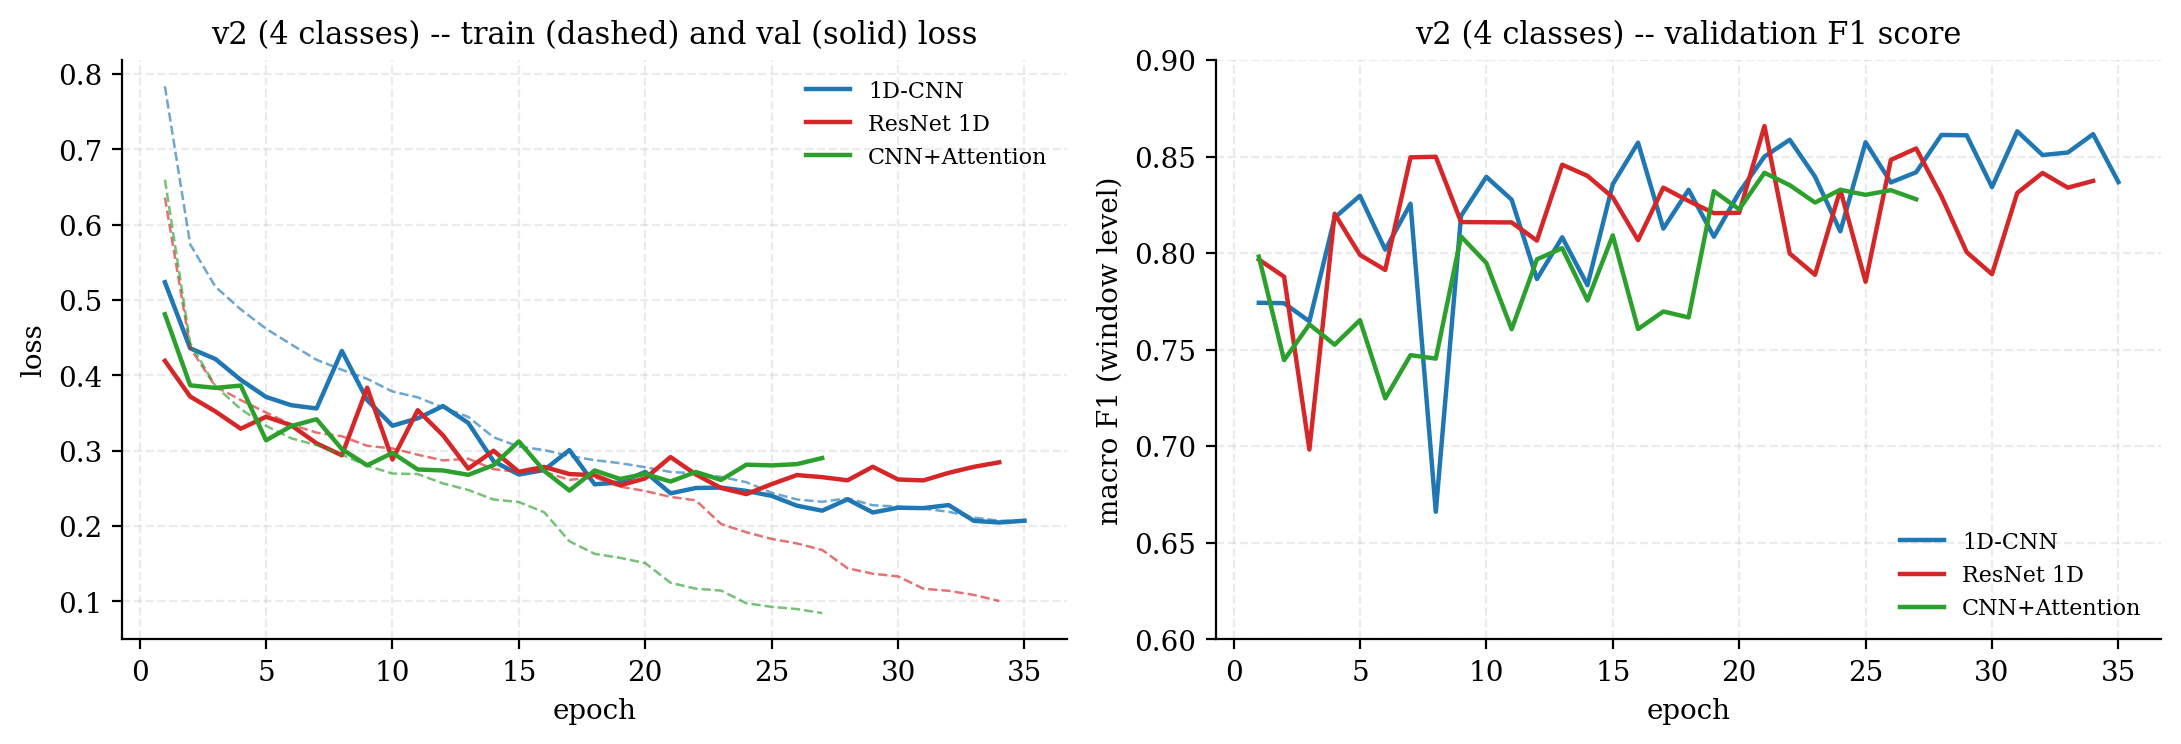
\includegraphics[width=\linewidth]{figures/v2_training_curves}
    \caption{v2 training dynamics. Left: train (dashed) and validation
    (solid) loss. Right: validation macro F1 (window level).}
    \label{fig:v2-training}
\end{figure}

\begin{itemize}[leftmargin=*, itemsep=0.25em]
    \item All three models converge well within $35$ epochs; the
    ResNet and the CNN+Attention model hit the early-stopping criterion
    a few epochs earlier than the 1D-CNN.
    \item Validation losses are lower than in v1 (the residual reaches
    $\sim 0.24$ vs $\sim 0.57$ in v1, the 1D-CNN reaches $\sim 0.21$ vs
    $\sim 0.73$). This is mostly a consequence of the simpler
    classification task --- four classes against seven, with the
    majority \texttt{Normal} class being trivial to separate from a
    bump.
    \item The validation F1 saturates around $0.85$--$0.87$ for all
    three models. The remaining $13$--$15\%$ are mostly window-level
    boundary effects: a $512$-sample window that contains $\sim 10\%$
    of a short event can flip between the anomaly and \texttt{Normal}
    labels depending on the windowing offset.
\end{itemize}

\section{Window-level test performance}
\label{sec:res-window}

After training, each model's best checkpoint is loaded and evaluated
on the held-out test windows. \Cref{tab:test-window} reports the
overall accuracy and the per-class accuracy.

\begin{table}[H]
    \centering
    \footnotesize
    \begin{tabular}{lccc}
        \toprule
        Class & \textbf{1D-CNN} & \textbf{ResNet 1D} & \textbf{CNN+Attention} \\
        \midrule
        \texttt{Normal Background} & $0.972$ & $0.972$ & $0.944$ \\
        \texttt{bell}              & $0.809$ & $0.858$ & $0.820$ \\
        \texttt{fast\_ascend}      & $0.800$ & $0.854$ & $0.856$ \\
        \texttt{fast\_descend}     & $0.659$ & $0.778$ & $0.789$ \\
        \midrule
        \textbf{Overall accuracy}  & $0.956$ & $0.961$ & $0.934$ \\
        \bottomrule
    \end{tabular}
    \caption{Window-level accuracy on the held-out v2 test set
    ($62\,485$ windows). \texttt{fast\_descend} is the hardest class
    on all three models --- short events on the falling edge are
    easily confused with windowing-induced boundary residue.}
    \label{tab:test-window}
\end{table}

\section{Event-level results}
\label{sec:res-event}

The window-level numbers in \cref{tab:test-window} are misleading at
the operational level for the same reason as in v1: a window is
labelled by majority anomaly content and the boundary windows of an
event flip between the anomaly class and \texttt{Normal} easily. The
right metric is event-level (\cref{sec:event-eval}), computed on a
continuous $100\,000$-sample segment.

On that segment the v2 generator places only $15$ ground-truth events
(against $59$ in the v1 dataset, an immediate consequence of the
density change). The event-level confusion matrices for the three
models are shown in \cref{fig:v2-confmat}.

\begin{figure}[H]
    \centering
    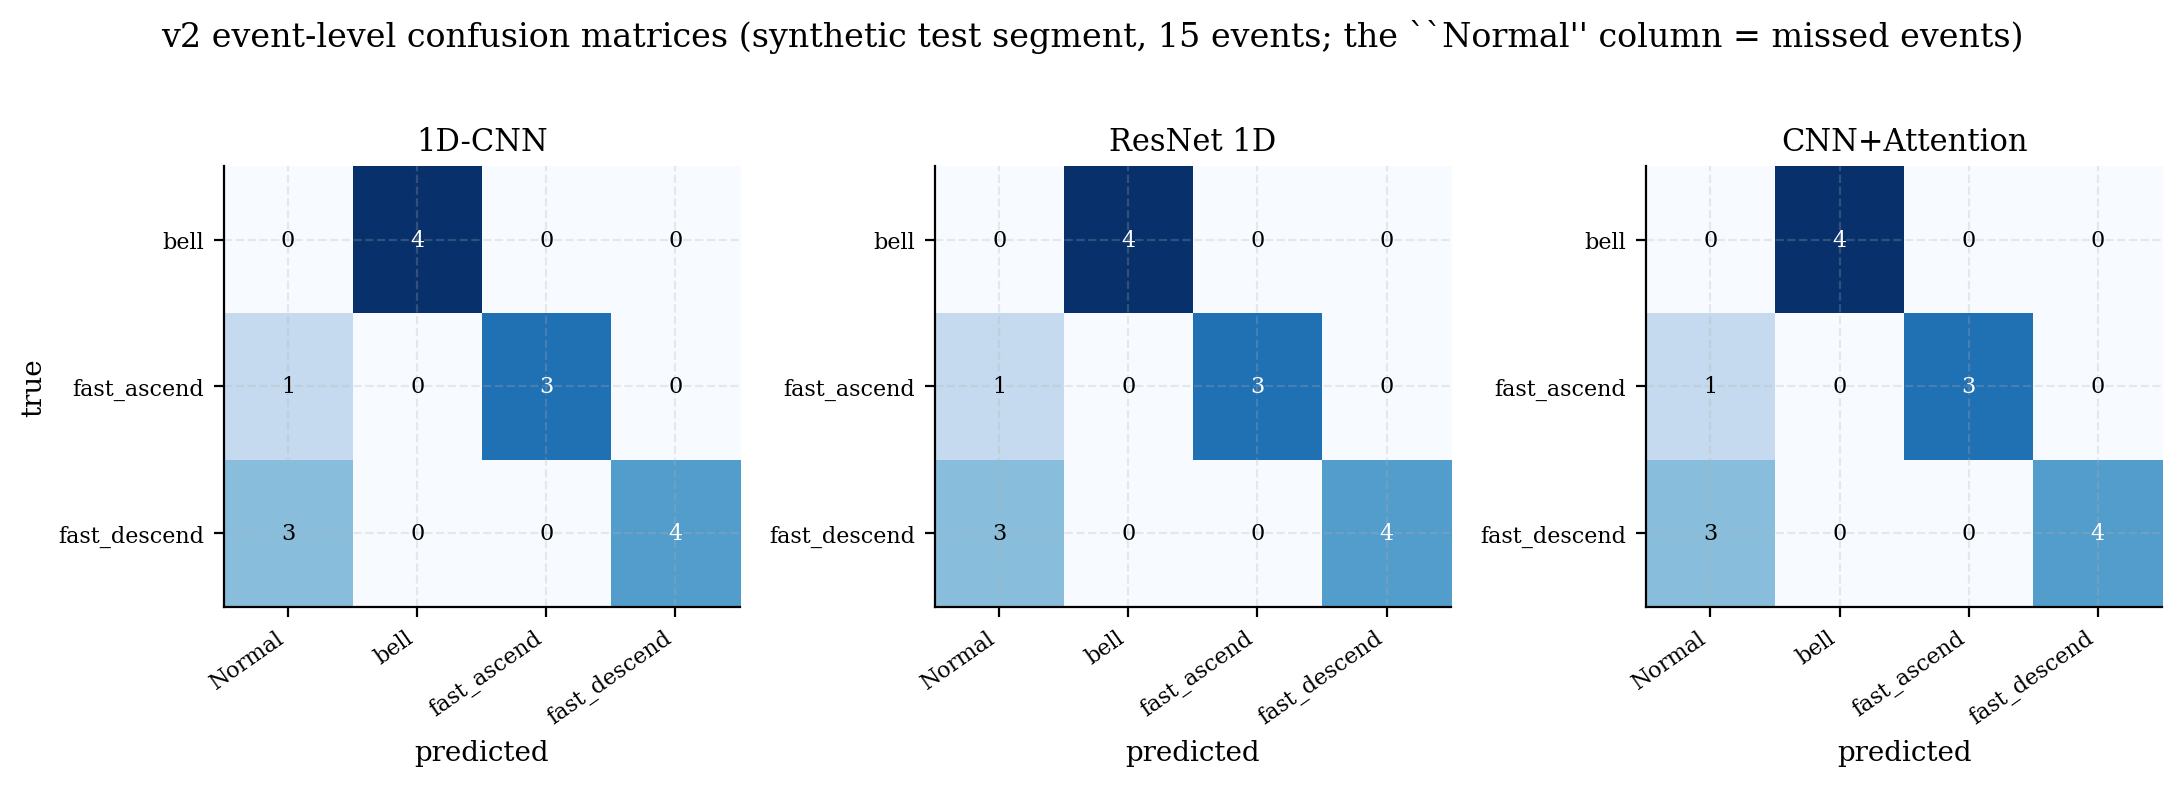
\includegraphics[width=\linewidth]{figures/v2_confusion_matrices}
    \caption{v2 event-level confusion matrices on the synthetic test
    segment. The leftmost column of each panel is the ``missed event''
    column --- a true event that has no overlapping prediction. All
    three models miss the same $4$ events (out of $15$): one
    \texttt{fast\_ascend} and three \texttt{fast\_descend}, all of
    them short events at the borderline duration of the detection
    threshold.}
    \label{fig:v2-confmat}
\end{figure}

The per-class precision/recall/F1 are summarised in
\cref{tab:v2-event-prf}.

\begin{table}[H]
    \centering
    \footnotesize
    \setlength{\tabcolsep}{4pt}
    \begin{tabular}{l ccc ccc ccc}
        \toprule
        & \multicolumn{3}{c}{\textbf{1D-CNN}} & \multicolumn{3}{c}{\textbf{ResNet 1D}} & \multicolumn{3}{c}{\textbf{CNN+Attention}} \\
        \cmidrule(lr){2-4}\cmidrule(lr){5-7}\cmidrule(lr){8-10}
        Class & P & R & F1 & P & R & F1 & P & R & F1 \\
        \midrule
        \texttt{bell}         & 1.00 & 1.00 & 1.00 & 1.00 & 1.00 & 1.00 & 1.00 & 1.00 & 1.00 \\
        \texttt{fast\_ascend} & 1.00 & 0.75 & 0.86 & 1.00 & 0.75 & 0.86 & 1.00 & 0.75 & 0.86 \\
        \texttt{fast\_descend}& 1.00 & 0.57 & 0.73 & 1.00 & 0.57 & 0.73 & 1.00 & 0.57 & 0.73 \\
        \midrule
        \textbf{Macro avg.}   & \textbf{1.00} & \textbf{0.77} & \textbf{0.86} & \textbf{1.00} & \textbf{0.77} & \textbf{0.86} & \textbf{1.00} & \textbf{0.77} & \textbf{0.86} \\
        \bottomrule
    \end{tabular}
    \caption{v2 per-class precision (P), recall (R) and F1 at the event
    level. All three models cluster around a $\sim 86\%$ macro F1 ---
    the four missed events are the same on all three models and
    correspond to the very short ($<60$-sample) end of the duration
    distribution, where the detection-driven event extractor
    (\cref{sec:event-eval}) loses sensitivity.}
    \label{tab:v2-event-prf}
\end{table}

\paragraph{Why all three models score the same.} The four missed
events are extremely short ($26$, $30$, $45$, $28$ samples) and sit
near the lower bound of the v2 duration range. With a sliding-window
stride of $10$ and a window length of $512$, an event shorter than
$\sim 50$ samples occupies only $\lesssim 10\%$ of the windows that
overlap it --- right at the labelling threshold of
\cref{sec:framing}. Sub-threshold events are silently mapped to
\texttt{Normal Background} by the per-window labelling rule, so the
network is not given a chance to predict the class. This is a feature
of the event extractor, not of the three architectures.

\paragraph{Precision and false positives.} Precision is $1.00$ for all
three models on all three classes: the v2 networks do not hallucinate.
On the synthetic test segment this is exactly what we want.

\section{Cost--performance comparison}
\label{sec:res-cost}

\Cref{fig:model-cost} summarises the cost/performance trade-off across
the three architectures on the v2 setup.

\begin{figure}[H]
    \centering
    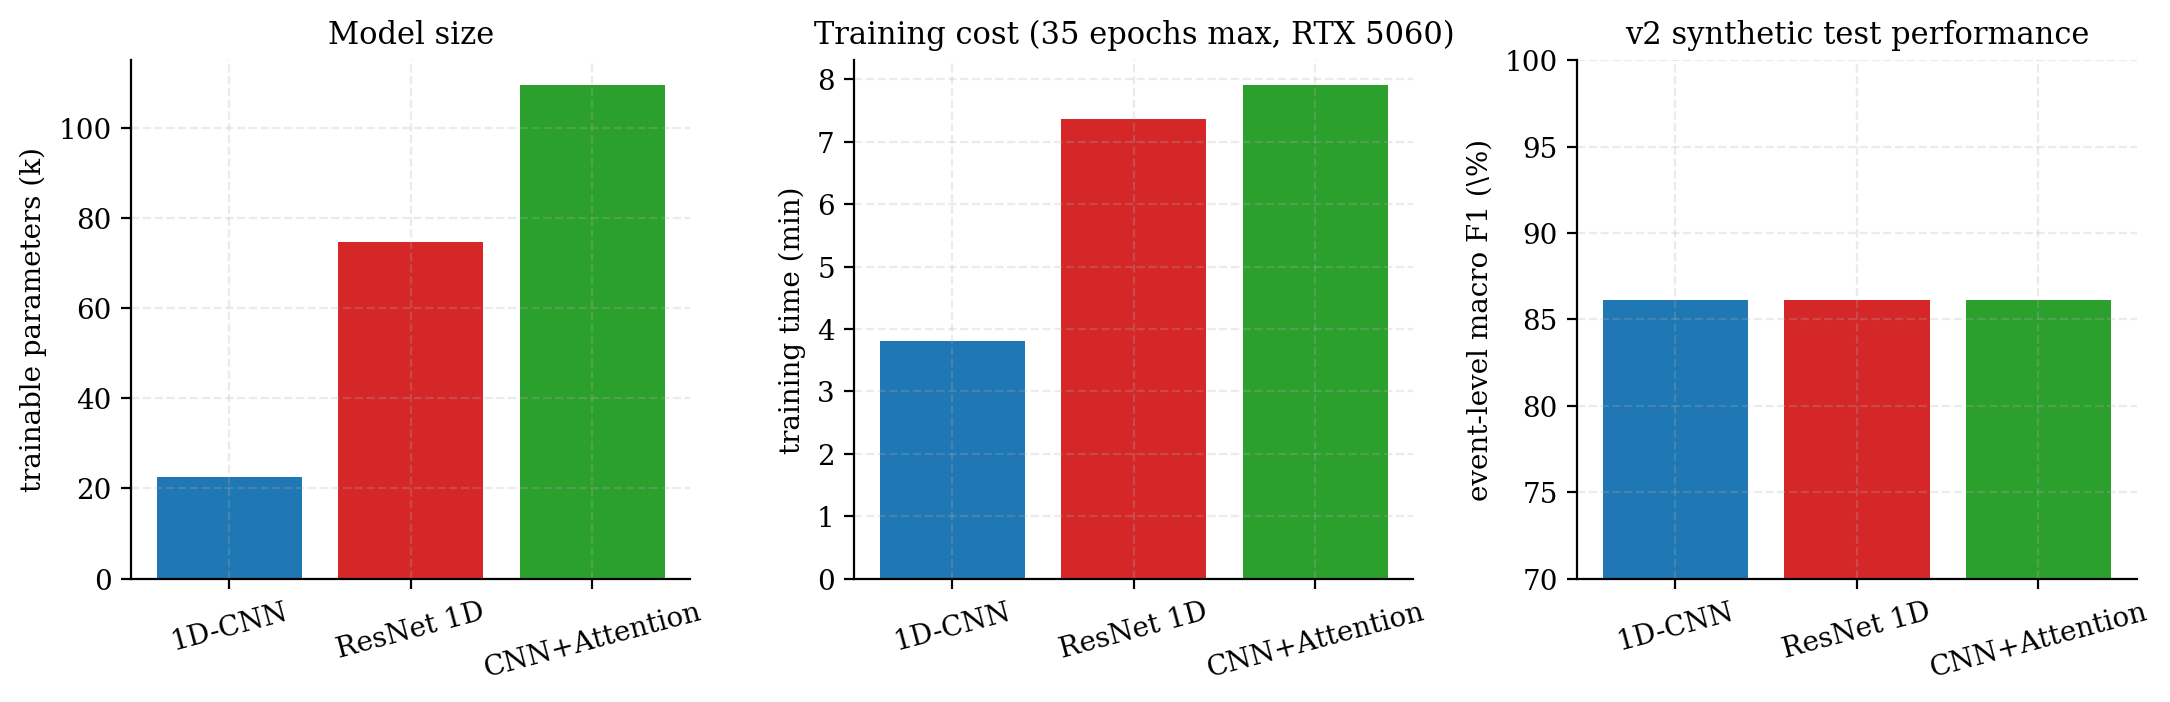
\includegraphics[width=\linewidth]{figures/model_cost}
    \caption{v2 cost--performance trade-off. \textbf{Left}: parameter
    count. \textbf{Centre}: total training time on a single RTX 5060
    Laptop GPU (the 1D-CNN ran the full $35$ epochs; the other two
    triggered early stopping after $\sim 27$ epochs). \textbf{Right}:
    event-level macro F1 on the synthetic test segment. Because the
    three networks converge to the same set of detected events on this
    segment, the F1 bars are equal.}
    \label{fig:model-cost}
\end{figure}

On v2 the three architectures are essentially tied at the event level
on the synthetic test set. The picture changes when we move to
robustness sweeps (\cref{chap:robustness}) and to the real-data
inference (\cref{chap:v2real}), where the differences in the
architectures' inductive biases re-emerge.
